\documentclass{tpu-sotu}
\usepackage{ascmac}
\usepackage{cite}
\usepackage[dvipdfmx]{hyperref}
\usepackage[dvipdfmx]{graphicx}
\usepackage{pxjahyper}
\usepackage{listings}%begin{lstlisting}で使える
\lstset{
basicstyle={\small},% 
identifierstyle={\small},% 
commentstyle={\small\ttfamily \color[rgb]{0,0,0}},% 
keywordstyle={\small\bfseries \color[rgb]{0,0,1}},% 
ndkeywordstyle={\small},% 
stringstyle={\small\ttfamily}, 
frame={tb}, 
breaklines=true, 
columns=[l]{fullflexible},% 
numbers=left,%これ消すと行番号消える
xrightmargin=0zw,% 
xleftmargin=3zw,% 
numberstyle={\scriptsize},% 
stepnumber=1, 
numbersep=1zw,% 
morecomment=[l]{//}% 
}

\title{UPPAALを用いた自動運転車の\\群制御アルゴリズムのモデル化と検証}
\etitle{title}
\author{佐原優衣}
\gakusekibangou{1515024}
\date{2019年2月}
\professor{中村 正樹 准教授}
\department{電子・情報工学科}
%- - - - - - - - - - - - - - - - - - - - - - - - -
\begin{document}
\maketitle
\clearpage
\pagenumbering{roman}
\setcounter{tocdepth}{3}
\tableofcontents
\clearpage
\pagenumbering{arabic}

\chapter{はじめに}
	\section{背景}
	移動手段として自動車はよく使われる。自動車の交通整備の方法として信号機が広く採用されている。しかし,交通量が少ない場所では信号機は導入されていないこともある。人が運転する場合は周囲に他車がいないこと,歩行者などがいないことを確認して通過する。では,自動運転車の場合を考える。
		\subsection{問題提起}
		街の中で多数の自動運転車が他車を考慮しない経路選択をすると問題が発生する恐れがある。そのためには個々による車の制御だけでなく群制御アルゴリズムを導入する必要があるだろう
	\section{目的}
	自動運転車の群制御アルゴリズムを形式的に記述し,モデル検査を用いて,性質を検証する。
	\section{論文の構成}
	本論文では,
\chapter{モデル検査}
本章では文献\cite{a1}からモデル検査とUPPAALの概説を行う。
	\section{モデル検査}
	モデル検査は,システム上で起こり得る状態を網羅的に調べることにより設計の誤りを発見する自動検証手法の一種である。モデル検査手法は,システムの振る舞いの設計,および検証したい性質をそれぞれモデル化し,ツールを用いて,システムが性質を満たしているかを調べる。
	
	モデル検査において,システムの動作を表現するシステムモデルを作成する必要がある。ソフトウェア開発のどの段階でモデル検査を活用したいか,もしくは,何をどの程度検証したいかによって,どのような情報をもとにどのようにシステムモデルを作成するかが変わってくる。専用のシステムモデルを入力とするモデル検査を設計モデル検査,ソースプログラムを入力とするモデル検査をプログラムモデル検査と呼ぶ。これらのモデル検査がソフトウェア開発の流れの中での活用例を図\ref{develP}に示す。図\ref{develP}にソフトウェアの品質向上のために行われる手順も挙げた。設計モデル検査は設計レビューを,プログラムモデル検査はコードレビューをそれぞれ補完する位置付けである。
	\subsection{様々なモデル検査ツール}
	次に,いくつかのモデル検査ツールを特徴と共に例示する。代表的なモデル検査ツールには,処理が高速で大規模なモデルを扱えるNuSMV,並列処理やマルチスレッドの設計モデルを扱えるSPIN,GUIベースの入力による時間制約を扱えるUPPAALなどがある。
	
	NuSMVは状態遷移図からのモデル化に向いており,また,各状態が満たす論理式などを用いて記号的に検査を行う,莫大な状態数を持つ系に対して検査が可能なシンボリックモデル検査ツールである。
	
	SPINはPromelaという専用の言語を用いて検証対象をモデル化する。動作主体を複数定義し,各動作主体の動作はC言語に似た文法で記述される。複数の動作主体の状態の組み合わせの数は,例え一動作主体あたりの状態数が比較的少なくとも,非常に大きくなることが起こりがちである。これを状態爆発と称される。SPINは状態爆発を緩和するために,半順序簡約,ビットステートハッシュ,状態ベクトル圧縮,データフロー・制御フロー解析によるスライシングなどの諸技術が用いられている。
	
	時間が扱える設計モデル検査の利点について述べる。イベントの発生時刻や処理時間,これらの時間的なズレの三点について任意に設定できるため,時間が扱えないモデル検査と違い,応答時間などの時間制約を検証対象にすることが可能である。また,イベントの発生と特定の処理の開始を簡単に記述できる。
	\begin{figure}[htbp]
	\centering
	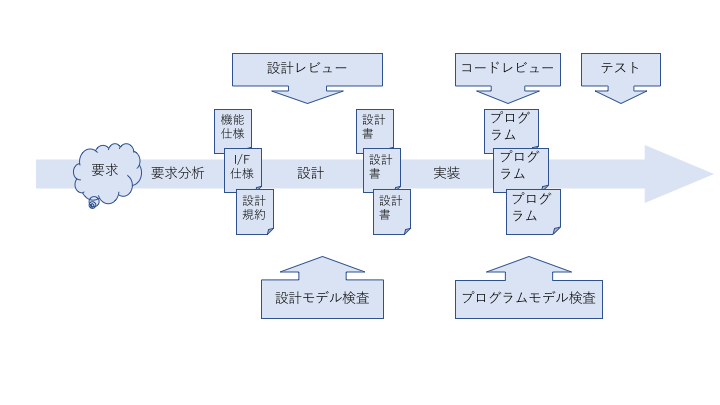
\includegraphics[width=160mm]{developmentProcess.png}
	\caption{ソフトウェア開発プロセス}
	\label{develP}
	\end{figure}

	\section{モデル検査ツールUPPAAL}
	本節は,UPPAALについて概説する。
	
	UPPAALはシステムモデルの入力をGUIベースにより定義している。このため,作成したシステムモデルが直感的に把握しやすい。入力したシステムモデルに対して,GUIベースでシミュレーション実行とステップ実行が可能である。シミュレーション画面では,各プロセスの現在状態と変数の値,状態遷移図とメッセージシーケンスが表示される。
	
	検証は検証したい性質を検証式で入力する。検証はすべての可能性のある実行パスに対して網羅的に検査を行う。検証結果は,入力した検証式に対して成否が緑か赤で示される。性質に反した場合は,反するまでの実行履歴が反例として示される。反例の表示はシミュレーション画面で行われ,ステップ単位でトレースすることで,各プロセスの状態や変数値の変化を確認可能である。
	また時間制約を含む検証に関して,「最短時間で違反状態に到達する反例の出力」という機能を持つ。通常出力されるのは任意の一種類ではあるが,特に初期状態から検証したい性質に反するまでの経過時間が最短となる反例を出力する機能である。検証したい性質として,「仕事が完了することがない」という条件を与えることにより,仕事が完了する手順が反例となるが,仕事が完了する手順の中で最短時間のものを出力することになる。
	
\chapter{群制御アルゴリズムの\\モデル化と検証}
	\section{モデル化}
	\section{検証}
\chapter{考察}
\chapter{おわりに}
\acknowledgements
\begin{thebibliography}{1}
	\bibitem{a1}{長谷川哲夫,田原康之,磯部祥尚,UPPAALによる性能モデル検証ーリアルタイムシステムのモデル化と検証ー,(株)近代科学社,2012.}
\end{thebibliography}
\end{document}